\documentclass[12pt]{article}

\usepackage[paper=letterpaper,margin=2cm]{geometry}

% images
\usepackage{graphicx}
\graphicspath{ {./images/} }
\usepackage{float}

% multiple text columns
% \usepackage{multicol}

% graphs
% good tutorial: https://latexdraw.com/how-to-draw-venn-diagrams-in-latex/
\usepackage{tikz}

% arrows
\usetikzlibrary{arrows.meta}

% matrices
\usepackage{amsmath}


\title{Graph theory}
\author{Author: Daniel Gigliotti}
% \date{\today}
\date{}


\begin{document}
\maketitle

\section{Graphs}

You know what a graph is

\begin{center}
	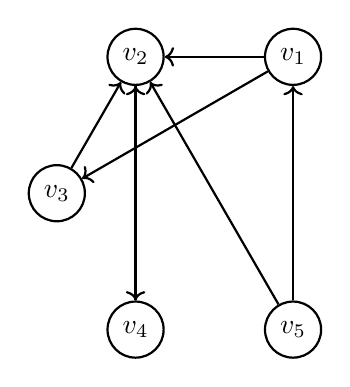
\begin{tikzpicture}[thick, main/.style = {draw, circle}] 
		\foreach \phi in {1,...,5}{
			\node[main] (v_\phi) at (360/6 * \phi:2cm) {$v_\phi$};
		}

		% The parameters sloped and pos indicate, respectively, that we want the weight to be orthogonal to the edge
		% and shifted by a certain amount along the edge.
		% \draw[->] (v_1) -- node[midway, above right, sloped, pos=0.85] {+1} (v_2);

		\draw[->] (v_1) -- (v_2);
		\draw[->] (v_5) -- (v_1);
		\draw[->] (v_5) -- (v_2);
		\draw[->] (v_1) -- (v_3);
		\draw[->] (v_3) -- (v_2);
		\draw[->] (v_4) -- (v_2);
		\draw[->] (v_2) -- (v_4);

	\end{tikzpicture}
\end{center}

\noindent
We can describe this graph with an $adjacency\ matrix$:

\begin{center}
	$A = \begin{bmatrix}
	0 & 0 & 0 & 0 & 1\\
	1 & 0 & 1 & 1 & 1\\
	1 & 0 & 0 & 0 & 0\\
	0 & 1 & 0 & 0 & 0\\
	0 & 0 & 0 & 0 & 0
	\end{bmatrix}$
\end{center}

\noindent
If the graph is undirected, the adjacency matrix is symmetric (duh) and we can consider only the upper (or lower) triangle.

\noindent
If the graph is directed, the adjacency matrix is not symmetric.

\section{Density}

The density $L$ of a graph is the ratio between the number of edges L in the graph and the maximum possible number of edges $L_{tot}$

\begin{center}
	$k = L/L_{tot}$
\end{center}

\begin{itemize}

	\item $ L_{tot} = \frac{N(N-1)}{2} $ for $undirected$ graphs (half adjacency matrix)
	\item $ L_{tot} = N(N-1) $ for $directed$ graphs (full adjacency matrix)

\end{itemize}

\noindent
The density for the above graph is $L_{tot} = N(N - 1) = 5(4) = 20$

\section{Degree}

The degree $g$ of a node $i$ ($i \in [1, N]$, $N$ = number of nodes in the graph) is the number of edges connected to that node:

\begin{center}
	$g_i = \sum_{j=0, j \neq i}^{N - 1} a_{ij}$ \\
	\vspace{20px}
	with $g_i \in [0, N - 1]$
\end{center}

\noindent
If the graph is directed:

\begin{itemize}
	\item in-degree of a node $i$ ($i \in [0, N - 1]$) is the number of edges directed to node $i$
	\item out-degree of a node $i$ ($i \in [0, N - 1]$) is the number of edges originated from node $i$
	\item degree of a node $i$ ($i \in [0, N - 1]$) is the number of edges originated from and directed to node $i$

	\begin{center}
		$g_i = g_i^{in} + g_i^{out}$ \\
		\vspace{20px}
		with $g_i \in [0, 2(N - 1)]$
	\end{center}
	
\end{itemize}

\noindent
If we want to compute the degrees for each node:

\vspace{20px}

\begin{minipage}[t]{0.3\textwidth}
	\begin{center}
			out-degree \\
			\vspace{20px}
			$g_1^{out} = 2$ \\
			$g_2^{out} = 1$ \\
			$g_3^{out} = 1$ \\
			$g_4^{out} = 1$ \\
			$g_5^{out} = 2$
	\end{center}
\end{minipage}\hfill
\begin{minipage}[t]{0.3\textwidth}
	\begin{center}
		in-degree \\
		\vspace{20px}
		$g_1^{in} = 1$ \\
		$g_2^{in} = 4$ \\
		$g_3^{in} = 1$ \\
		$g_4^{in} = 1$ \\
		$g_5^{in} = 0$
	\end{center}    
\end{minipage}\hfill
\begin{minipage}[t]{0.3\textwidth}
	\begin{center}
		degree \\
		\vspace{20px}        
		$g_1 = 3$ \\
		$g_2 = 5$ \\
		$g_3 = 2$ \\
		$g_4 = 2$ \\
		$g_5 = 2$
	\end{center}
\end{minipage}

\newpage

\section{Path}

A $path$ is any possible sequence of edges linking two nodes. The $path\ length$ is given by the number of edges from which the path is composed.

\vspace{20px}

\begin{minipage}[t]{0.3\textwidth}
	\begin{center}
		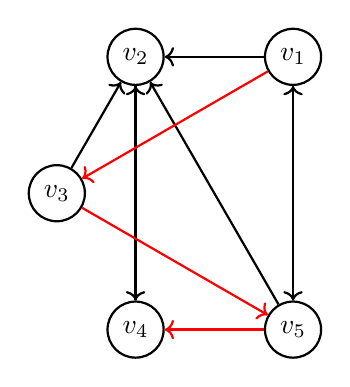
\begin{tikzpicture}[thick, main/.style = {draw, circle}] 
			\foreach \phi in {1,...,5}{
				\node[main] (v_\phi) at (360/6 * \phi:2cm) {$v_\phi$};
			}
	
			% The parameters sloped and pos indicate, respectively, that we want the weight to be orthogonal to the edge
			% and shifted by a certain amount along the edge.
			% \draw[->] (v_1) -- node[midway, above right, sloped, pos=0.85] {+1} (v_2);
	
			\draw[->] (v_1) -- (v_2);
			\draw[->] (v_1) -- (v_5);
			\draw[->] (v_5) -- (v_1);
			\draw[->] (v_5) -- (v_2);
			\draw[->] (v_3) -- (v_2);
			\draw[->] (v_4) -- (v_2);
			\draw[->] (v_2) -- (v_4);
   			\draw[->,draw=red] (v_1) -- (v_3);
			\draw[->,draw=red] (v_3) -- (v_5);
			\draw[->,draw=red] (v_5) -- (v_4);
	
		\end{tikzpicture}
	\end{center}
\end{minipage}\hfill
\begin{minipage}[t]{0.3\textwidth}
	\begin{center}
		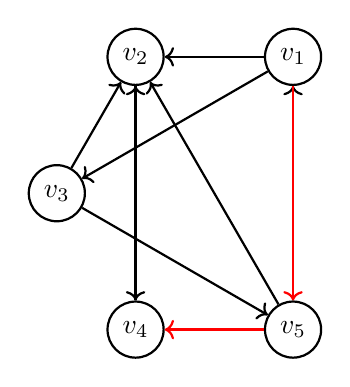
\begin{tikzpicture}[thick, main/.style = {draw, circle}] 
			\foreach \phi in {1,...,5}{
				\node[main] (v_\phi) at (360/6 * \phi:2cm) {$v_\phi$};
			}
	
			% The parameters sloped and pos indicate, respectively, that we want the weight to be orthogonal to the edge
			% and shifted by a certain amount along the edge.
			% \draw[->] (v_1) -- node[midway, above right, sloped, pos=0.85] {+1} (v_2);
	
			\draw[->] (v_1) -- (v_2);
			\draw[->] (v_5) -- (v_1);
			\draw[->] (v_5) -- (v_2);
			\draw[->] (v_1) -- (v_3);
			\draw[->] (v_3) -- (v_2);
			\draw[->] (v_4) -- (v_2);
			\draw[->] (v_2) -- (v_4);
			\draw[->] (v_3) -- (v_5);
   			\draw[->,draw=red] (v_1) -- (v_5);
			\draw[->,draw=red] (v_5) -- (v_4);
	
		\end{tikzpicture}
	\end{center}    
\end{minipage}\hfill
\begin{minipage}[t]{0.3\textwidth}
	\begin{center}
		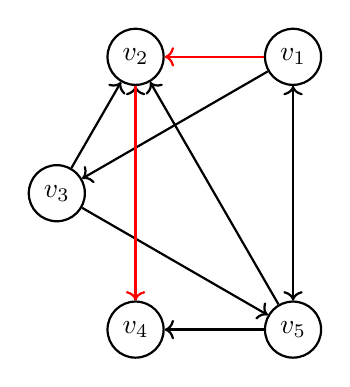
\begin{tikzpicture}[thick, main/.style = {draw, circle}] 
			\foreach \phi in {1,...,5}{
				\node[main] (v_\phi) at (360/6 * \phi:2cm) {$v_\phi$};
			}
	
			% The parameters sloped and pos indicate, respectively, that we want the weight to be orthogonal to the edge
			% and shifted by a certain amount along the edge.
			% \draw[->] (v_1) -- node[midway, above right, sloped, pos=0.85] {+1} (v_2);
	
			\draw[->] (v_1) -- (v_5);
			\draw[->] (v_5) -- (v_1);
			\draw[->] (v_5) -- (v_2);
			\draw[->] (v_1) -- (v_3);
			\draw[->] (v_3) -- (v_2);
			\draw[->] (v_4) -- (v_2);
			\draw[->] (v_3) -- (v_5);
			\draw[->] (v_5) -- (v_4);
			\draw[->,draw=red] (v_1) -- (v_2);
			\draw[->,draw=red] (v_2) -- (v_4);

		\end{tikzpicture}
	\end{center}
\end{minipage}

\vspace{20px}

\begin{center}
	3 paths linking $v_1$ to $v_4$
	\item $v_1 \rightarrow v_3 \rightarrow v_5 \rightarrow v_4\ (3 steps)$
	\item $v_1 \rightarrow v_5 \rightarrow v_4\ (2 steps)$
	\item $v_1 \rightarrow v_2 \rightarrow v_4\ (2 steps)$
\end{center}

\section{Distance}

$Distance\ d(i, j)$ between nodes $i$ and $j$ is the $shortest\ path$ between them

\vspace{20px}

\begin{center}
	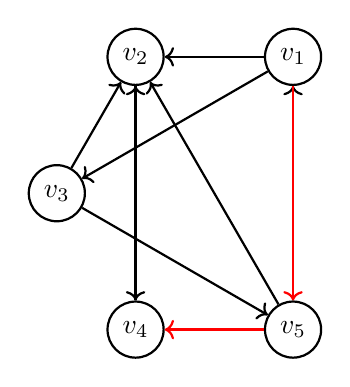
\begin{tikzpicture}[thick, main/.style = {draw, circle}] 
		\foreach \phi in {1,...,5}{
			\node[main] (v_\phi) at (360/6 * \phi:2cm) {$v_\phi$};
		}

		% The parameters sloped and pos indicate, respectively, that we want the weight to be orthogonal to the edge
		% and shifted by a certain amount along the edge.
		% \draw[->] (v_1) -- node[midway, above right, sloped, pos=0.85] {+1} (v_2);

		\draw[->] (v_1) -- (v_2);
		\draw[->] (v_5) -- (v_1);
		\draw[->] (v_5) -- (v_2);
		\draw[->] (v_1) -- (v_3);
		\draw[->] (v_3) -- (v_2);
		\draw[->] (v_4) -- (v_2);
		\draw[->] (v_2) -- (v_4);
		\draw[->] (v_3) -- (v_5);
  		\draw[->,draw=red] (v_1) -- (v_5);
		\draw[->,draw=red] (v_5) -- (v_4);

	\end{tikzpicture}

	\vspace{20px}

	$v_1 \rightarrow v_5 \rightarrow v_4\ (2 steps)$ \\
	$d(v_1, v_5) = 2 \rightarrow\ Shortest\ path\ between\ v_1\ and\ v_4$
	
\end{center}

We can even build a $distance\ matrix$

\begin{center}

    $D = \begin{bmatrix}
    0 & 1 & 1 & 2 & 1\\
    \infty & 0 & \infty & 1 & \infty\\
    2 & 1 & 0 & 2 & 1\\
    \infty & 1 & \infty & 0 & \infty\\
    1 & 1 & 2 & 1 & 0\\
    \end{bmatrix}$
    
\end{center}

\newpage

\section{Global efficiency}

The $global\ efficiency\ E_g$ of a graph is the average of the reciprocal of the distances between any pair of nodes. It measures how efficiently the information is exchanged in the network. 

\begin{center}
\vspace{20px}

$E_g = \frac{1}{N(N-1)} \sum_{i=0}^{N - 1} \sum_{j=0, j \neq i}^{N - 1} \frac{1}{d_{ij}}\ $ for directed graphs

\vspace{20px}

$E_g = \frac{2}{N(N-1)} \sum_{i=0}^{N - 1} \sum_{j=0, j \neq i}^{N - 1} \frac{1}{d_{ij}}\ $ for undirected graphs

\vspace{20px}

with $E_g \in [0, 1]$

\vspace{20px}
\end{center}

\noindent
In general:

\begin{center}
\vspace{20px}

$E_g = \frac{1}{L_{tot}} \sum_{i=0}^{N - 1} \sum_{j=0, j \neq i}^{N - 1} \frac{1}{d_{ij}}$

\end{center}

\newpage

\section{Local efficiency}

$Local\ efficiency$ measures the tendency of the network to form strongly connected subgroups. It is a measure of the robustness of the network to the removal of a node. For each node $i$ we can extract a subnetwork $S_i$ made of all the nodes directly connected to $i$ excluding $i$ itself and compute its global efficiency $E_g(S_i)$

\vspace{20px}

\noindent
Starting from this graph

\vspace{20px}

\begin{center}
	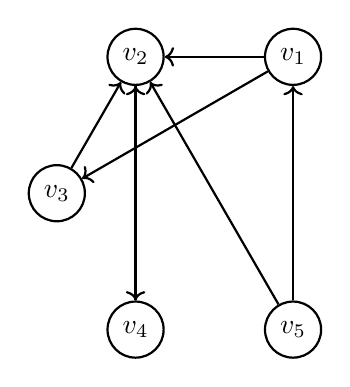
\begin{tikzpicture}[thick, main/.style = {draw, circle}] 
		\foreach \phi in {1,...,5}{
			\node[main] (v_\phi) at (360/6 * \phi:2cm) {$v_\phi$};
		}

		% The parameters sloped and pos indicate, respectively, that we want the weight to be orthogonal to the edge
		% and shifted by a certain amount along the edge.
		% \draw[->] (v_1) -- node[midway, above right, sloped, pos=0.85] {+1} (v_2);

		\draw[->] (v_1) -- (v_2);
		\draw[->] (v_5) -- (v_1);
		\draw[->] (v_5) -- (v_2);
		\draw[->] (v_1) -- (v_3);
		\draw[->] (v_3) -- (v_2);
		\draw[->] (v_4) -- (v_2);
		\draw[->] (v_2) -- (v_4);

	\end{tikzpicture}
\end{center}

\vspace{20px}

\noindent
We will have:

\vspace{20px}

\begin{minipage}[t]{0.3\textwidth}
	\begin{center}
		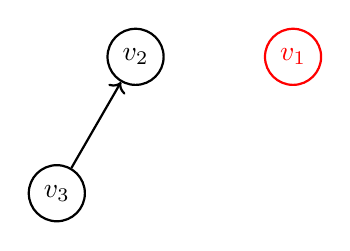
\begin{tikzpicture}[thick, main/.style = {draw, circle}, selected/.style = {draw, circle, color=red}] 

			\node[selected] (v_1) at (360/6 * 1:2cm) {$v_1$};
			
			\foreach \phi in {2,...,3}{
				\node[main] (v_\phi) at (360/6 * \phi:2cm) {$v_\phi$};
			}

			\draw[->] (v_3) -- (v_2);
	
		\end{tikzpicture}
		\\
		\vspace{20px}
		For $v_1$
	\end{center}
\end{minipage}\hfill
\begin{minipage}[t]{0.3\textwidth}
	\begin{center}
		
\begin{tikzpicture}[thick, main/.style = {draw, circle}, selected/.style = {draw, circle, color=red}] 
			
                \node[selected] (v_2) at (360/6 * 2:2cm) {$v_2$};
                \node[main] (v_4) at (360/6 * 4:2cm) {$v_4$};
	
		\end{tikzpicture}
            \\
		\vspace{20px}
		For $v_2$
	\end{center}    
\end{minipage}\hfill
\begin{minipage}[t]{0.3\textwidth}
	\begin{center}
            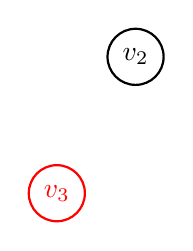
\begin{tikzpicture}[thick, main/.style = {draw, circle}, selected/.style = {draw, circle, color=red}] 
			
                \node[main] (v_2) at (360/6 * 2:2cm) {$v_2$};
                \node[selected] (v_3) at (360/6 * 3:2cm) {$v_3$};
   
		\end{tikzpicture}
            \\
		\vspace{20px}
		For $v_3$
	\end{center}
\end{minipage}

\vspace{30px}

\begin{minipage}[t]{0.45\textwidth}
	\begin{center}
		
\begin{tikzpicture}[thick, main/.style = {draw, circle}, selected/.style = {draw, circle, color=red}] 

			\node[selected] (v_4) at (360/6 * 4:2cm) {$v_4$};
                \node[main] (v_2) at (360/6 * 2:2cm) {$v_2$};
	
		\end{tikzpicture}
		\\
		\vspace{20px}
		For $v_4$
	\end{center}
\end{minipage}\hfill
\begin{minipage}[t]{0.45\textwidth}
	\begin{center}
		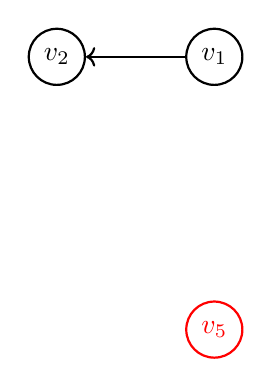
\begin{tikzpicture}[thick, main/.style = {draw, circle}, selected/.style = {draw, circle, color=red}] 
			
			\node[selected] (v_5) at (360/6 * 5:2cm) {$v_5$};
                \node[main] (v_1) at (360/6 * 1:2cm) {$v_1$};
                \node[main] (v_2) at (360/6 * 2:2cm) {$v_2$};

                \draw[->] (v_1) -- (v_2);

		\end{tikzpicture}
            \\
		\vspace{20px}
		For $v_5$
	\end{center}    
\end{minipage}\hfill

\begin{minipage}[t]{0.3\textwidth}
	\begin{center}
            $D = \begin{bmatrix}
            0 & \infty\\
            1 & 0
            \end{bmatrix}$
		\\
		\vspace{20px}
		For $v_1$
	\end{center}
\end{minipage}\hfill
\begin{minipage}[t]{0.3\textwidth}
	\begin{center}
            $D = \begin{bmatrix}
            0\\
            \end{bmatrix}$
            \\
		\vspace{20px}
		For $v_2$
	\end{center}    
\end{minipage}\hfill
\begin{minipage}[t]{0.3\textwidth}
	\begin{center}
            $D = \begin{bmatrix}
            0\\
            \end{bmatrix}$
            \\
		\vspace{20px}
		For $v_3$
	\end{center}
\end{minipage}

\vspace{30px}

\begin{minipage}[t]{0.45\textwidth}
	\begin{center}
            $D = \begin{bmatrix}
            0\\
            \end{bmatrix}$
		\\
		\vspace{20px}
		For $v_4$
	\end{center}
\end{minipage}\hfill
\begin{minipage}[t]{0.45\textwidth}
	\begin{center}
            $D = \begin{bmatrix}
            0 & 1\\
            \infty & 0
            \end{bmatrix}$
            \\
		\vspace{20px}
		For $v_5$
	\end{center}
\end{minipage}\hfill

\vspace{20px}

For some applications it may be interesting to measure how well a network can be divided into $communities$.

\vspace{20px}

\newcommand{\printlist}[1]{%
    \foreach \x [count=\xi] in {#1} {
        \xi. \x\par
    }%
}

\begin{center}
    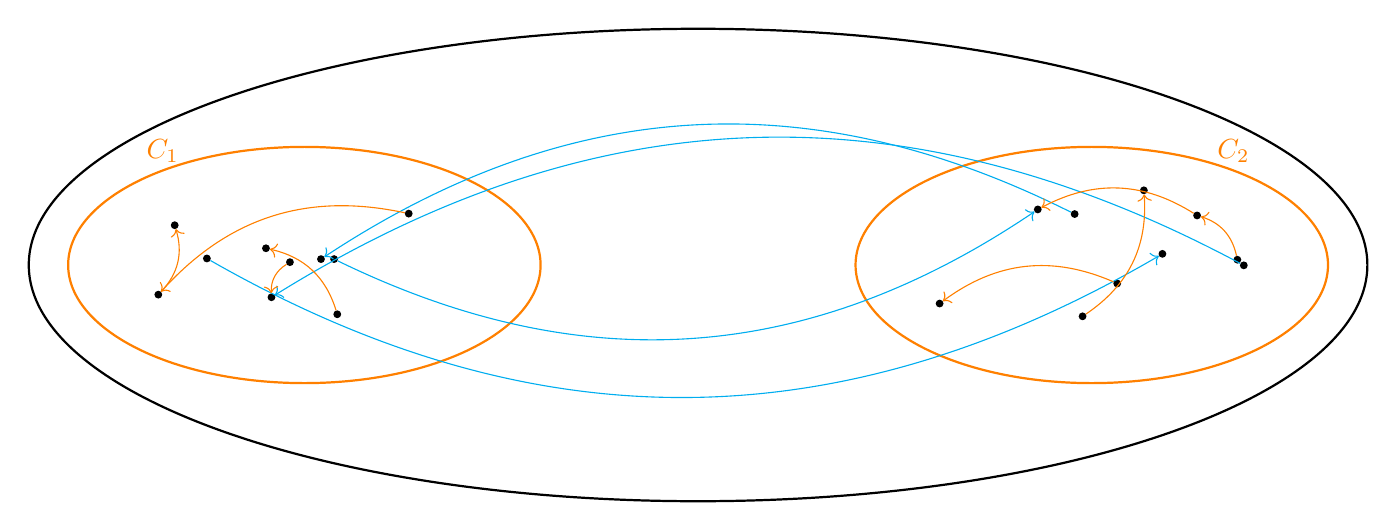
\begin{tikzpicture}

        % Set A
        \node [circle,
            fill=white,
            label={[orange]$C_1$}] (A) at (-1.8, 1){};

        % Set B
        \node [circle,
            fill=white,
            label={[orange]$C_2$}] (B) at (10 + 1.8, 1){};
        
        \draw[orange,thick] (0,0) ellipse (3 and 1.5); % size of ellipse defined by its radius
        \draw[orange,thick] (10,0) ellipse (3 and 1.5);

        \draw[black,thick] (5,0) ellipse (8.5 and 3);

        % draw some point inside C_1
        \node [circle, fill=black, scale=0.3] (A) at (-0.1835214600812738, 0.03606614541319697){};
        \node [circle, fill=black, scale=0.3] (B) at (-1.2379449522321648, 0.08284803546333297){};
        \node [circle, fill=black, scale=0.3] (C) at (0.21057146057585463, 0.07464162069619462){};
        \node [circle, fill=black, scale=0.3] (D) at (1.325186962883449, 0.6526925336560812){};
        \node [circle, fill=black, scale=0.3] (E) at (-1.8547199642087284, -0.3764907075156738){};
        \node [circle, fill=black, scale=0.3] (F) at (0.4177514391263424, -0.6255449230158633){};
        \node [circle, fill=black, scale=0.3] (G) at (-0.48790878816243577, 0.21246742194910073){};
        \node [circle, fill=black, scale=0.3] (H) at (-1.6467060183522997, 0.505183581567271){};
        \node [circle, fill=black, scale=0.3] (I) at (0.37762704411498715, 0.07503894950722656){};
        \node [circle, fill=black, scale=0.3] (J) at (-0.4177905764107237, -0.4094517716669088){};

        % draw some point inside C_1
        \node [circle, fill=black, scale=0.3] (K) at (10.322694946345393, -0.23437915046836322){};
        \node [circle, fill=black, scale=0.3] (L) at (8.067516762774416, -0.48941710301433794){};
        \node [circle, fill=black, scale=0.3] (M) at (11.84886382256429, 0.06722225392141823){};
        \node [circle, fill=black, scale=0.3] (N) at (11.930897933081452, -0.004340633729034149){};
        \node [circle, fill=black, scale=0.3] (O) at (9.883153834671615, -0.6519101873729803){};
        \node [circle, fill=black, scale=0.3] (P) at (10.661656950916697, 0.9483029555553188){};
        \node [circle, fill=black, scale=0.3] (Q) at (11.337440301970535, 0.6293613039044264){};
        \node [circle, fill=black, scale=0.3] (R) at (9.314159851383906, 0.7057023751748575){};
        \node [circle, fill=black, scale=0.3] (S) at (9.782435772967498, 0.6471469965866659){};
        \node [circle, fill=black, scale=0.3] (T) at (10.89699635148537, 0.14151736292264028){};
        
        % draw the arrows
        \path[cyan, ->] (B) edge[bend right] node [left] {} (T);
        \path[cyan, ->] (S) edge[bend right] node [left] {} (C);
        \path[cyan, ->] (I) edge[bend right] node [left] {} (R);
        \path[cyan, ->] (N) edge[bend right] node [left] {} (J);
        
        \path[orange, ->] (A) edge[bend right] node [left] {} (J);
        \path[orange, ->] (E) edge[bend right] node [left] {} (H);
        \path[orange, ->] (D) edge[bend right] node [left] {} (E);
        \path[orange, ->] (F) edge[bend right] node [left] {} (G);

        \path[orange, ->] (K) edge[bend right] node [left] {} (L);
        \path[orange, ->] (M) edge[bend right] node [left] {} (Q);
        \path[orange, ->] (O) edge[bend right] node [left] {} (P);
        \path[orange, ->] (Q) edge[bend right] node [left] {} (R);
        
    \end{tikzpicture}
\end{center}

\vspace{20px}

A subnetwork is a community if it shows an organized structure with respect to the entire network. Measures useful to determine if two or more subnetworks act as communities are the $divisibility$ and $modularity$.

\newpage

\section{Divisibility}

Divisibility $D$ is a measure of the segregation between two communities. It focuses on inter-community links.

\begin{center}

	$D = \frac{2L}{2L + \sum_{i, j = 0}^{N - 1}a_{ij}[1 - \delta (C_i, C_j)]}$ for $undirected$ graphs

	\vspace{20px}

	$D = \frac{L}{L + \sum_{i, j = 0}^{N - 1}a_{ij}[1 - \delta (C_i, C_j)]}$ for $directed$ graphs

	\vspace{20px}

	$D \in [\frac{1}{2}, 1]$

	\vspace{20px}

	$\begin{cases}
		
		\delta (C_i, C_j) = 1 if C_i == C_j \\

		\delta (C_i, C_j) = 0 otherwise

	\end{cases}$

	\vspace{20px}

	$\delta$ tells us if the two nodes belongs to the same community

	$L$ is the number of edges in the network

\end{center}

\newpage

\section{Modularity}

Modularity $Q$ measures the tendency of the subnetworks to form communities. It focuses on intra-community links.

\begin{center}

	$Q = \frac{1}{2L} \sum_{i, j = 0}^{N - 1}(a_{ij} - \frac{g_i g_j}{2L}) \delta (C_i, C_j)$ for $undirected$ graphs

	\vspace{20px}

	$Q = \frac{1}{L} \sum_{i, j = 0}^{N - 1}(a_{ij} - \frac{g_i^{in} g_j^{out}}{L}) \delta (C_i, C_j)$ for $directed$ graphs

	\vspace{20px}

	$\begin{cases}
		
		\delta (C_i, C_j) = 1 if C_i == C_j \\

		\delta (C_i, C_j) = 0 otherwise

	\end{cases}$

	\vspace{20px}

	$\delta$ tells us if the two nodes belongs to the same community

	$L$ is the number of edges in the network

\end{center}

For each pair of nodes belonging to the same community, modularity Q compares the existance (or not) of a link between them with the probability of having a connection between them in a random distribution of the links. 

\vspace{20px}

\begin{center}
	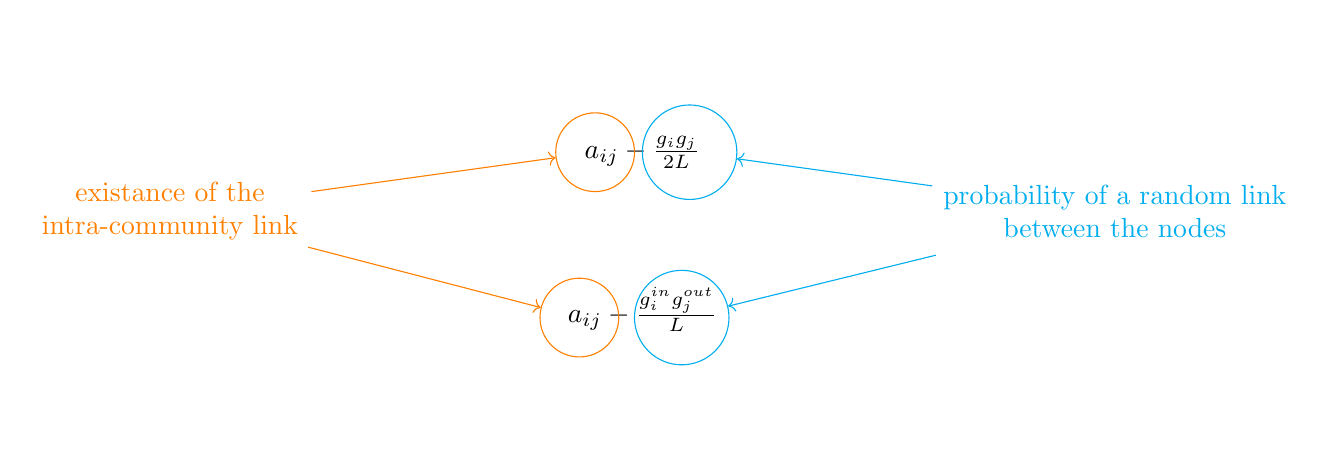
\begin{tikzpicture}

		\draw (-6, 0.25)
		node[align=center,minimum size=3cm,circle, text=orange] (A) 
		{existance of the \\ intra-community link};

		\draw (6, 0.25)
		node[align=center,minimum size=3cm,circle, text=cyan] (B)
		{probability of a random link \\ between the nodes};

		\draw (0, 1)
		node[align=center,minimum size=3cm,circle] (C)
		{$a_{ij} - \frac{g_i g_j}{2L}$};

		\draw (0, -1)
		node[align=center,minimum size=3cm,circle] (D)
		{$a_{ij} - \frac{g_i^{in} g_j^{out}}{L}$};

		\draw (-0.6, 1)
		node[align=center,minimum size=1cm,circle,draw=orange] (E)
		{};

		\draw (-0.8, -1.1)
		node[align=center,minimum size=1cm,circle,draw=orange] (F)
		{};

		\draw (0.6, 1)
		node[align=center,minimum size=1.2cm,circle,draw=cyan] (G)
		{};

		\draw (0.5, -1.1)
		node[align=center,minimum size=1.2cm,circle,draw=cyan] (H)
		{};

		\path[orange, ->] (A) edge[right] node [left] {} (E);
		\path[orange, ->] (A) edge[right] node [left] {} (F);

		\path[cyan, ->] (B) edge[right] node [left] {} (G);
		\path[cyan, ->] (B) edge[right] node [left] {} (H);

	\end{tikzpicture}
\end{center}

If there are more intra-community links than in a random division, Q $>$ 0, otherwise Q $\leq$ 0

\begin{center}
	\begin{tabular}{ c c }
		Integration	& Segregation \\
		\\
		\color{orange}	high	\color{black}	global efficiency & \color{cyan}	low		\color{black}	global efficiency \\
		\color{cyan}	low		\color{black}	global efficiency & \color{orange}	high	\color{black}	global efficiency \\
		\color{cyan}	low		\color{black}	global efficiency & \color{orange}	high	\color{black}	global efficiency \\
		\color{cyan}	low		\color{black}	global efficiency & \color{orange}	high	\color{black}	global efficiency \\
	\end{tabular}
\end{center}

\newpage

\section{Reference networks}

\vspace{20px}

\noindent
\begin{minipage}{0.3\textwidth}
	\includegraphics[scale=0.6]{images/regular_network.png}
\end{minipage}\hfill
\begin{minipage}{0.6\textwidth}
    Regular networks: each node is linked to a small number of other nodes. The degree is the same for all nodes. Efficient communications between small groups (high local efficiency), unefficient communication at the entire network level (low global efficiency).
\end{minipage}

\vspace{20px}

\noindent
\begin{minipage}{0.3\textwidth}
	\includegraphics[scale=0.6]{images/random_network.png} 
\end{minipage}\hfill
\begin{minipage}{0.6\textwidth}
	Random networks: each node is linked to the others randomly. There are no small groups with a strong internal communication (high global efficiency, low local efficiency).
\end{minipage}

\vspace{20px}

Those two are ideal cases: real networks are neither like the random nor like the regular graphs. 

\begin{center}
	\includegraphics[scale=0.4]{images/real_network.png}
\end{center}

\begin{center}
	$ E_g (Regular)\ <\ E_g(Small-world)\ <\ E_g(Random)$
	$ E_l (Random)\ <\ E_l(Small-world)\ <\ E_l(Regular)$
\end{center}

\end{document}
